\documentclass[12pt, a4paper]{article}
\usepackage[UTF8]{ctex}
\usepackage{amsmath}
\usepackage{amssymb}
\usepackage{amsthm}
\usepackage{geometry}
\usepackage{enumitem}
\usepackage{indentfirst}
\usepackage{caption}
\usepackage{fancyhdr}
\usepackage{booktabs}
\usepackage{titlesec}
\usepackage{draftwatermark}%水印
\usepackage{graphicx} % 导入图像的宏包、单图
% 页面布局设置
\geometry{top=2.54cm, bottom=2.54cm, left=3.18cm, right=3.18cm}

\SetWatermarkText{B站：布加拉提}
\SetWatermarkScale{0.4}

% 行距设置
\linespread{1.5}

% 段落设置
\setlength{\parindent}{2em}
\setlength{\parskip}{0.5em}

% 节标题格式设置
\titleformat{\section}{\normalfont\Large\bfseries}{第\chinese{section}章、}{1em}{}
\titlespacing{\section}{0pt}{2.5ex plus 1ex minus .2ex}{1.3ex plus .2ex}

% 定理环境设置
\newtheoremstyle{solution}
{}
{}
{}
{}
{\bfseries}
{、}
{1em}
{}
\theoremstyle{solution}
\newtheorem{sol}{解}

% 页眉页脚设置
\pagestyle{fancy}
\fancyhf{}
\fancyhead[C]{b站布加拉提整理（回忆版）b站甘茶w独家讲解}
\fancyfoot[C]{\thepage}

\rfoot{整理人：八方\\资源提供：考研乔瑟夫}
\lhead{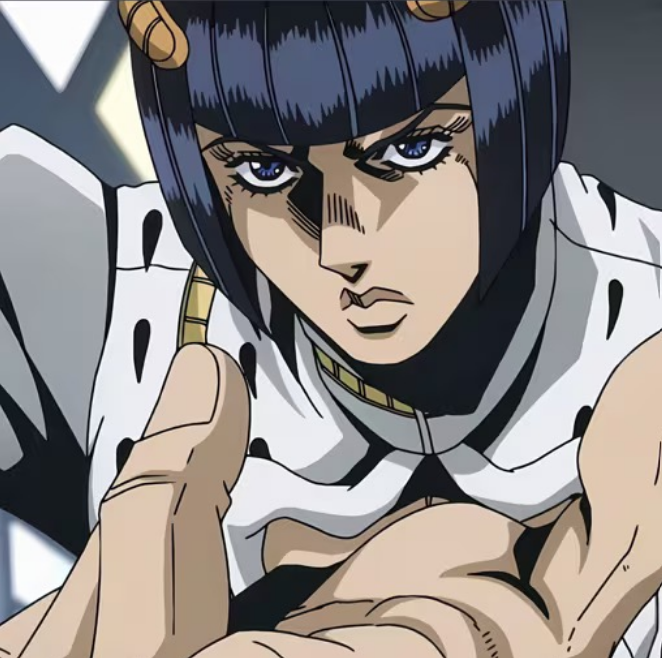
\includegraphics[width=0.06\linewidth]{p1.png}}
\rhead{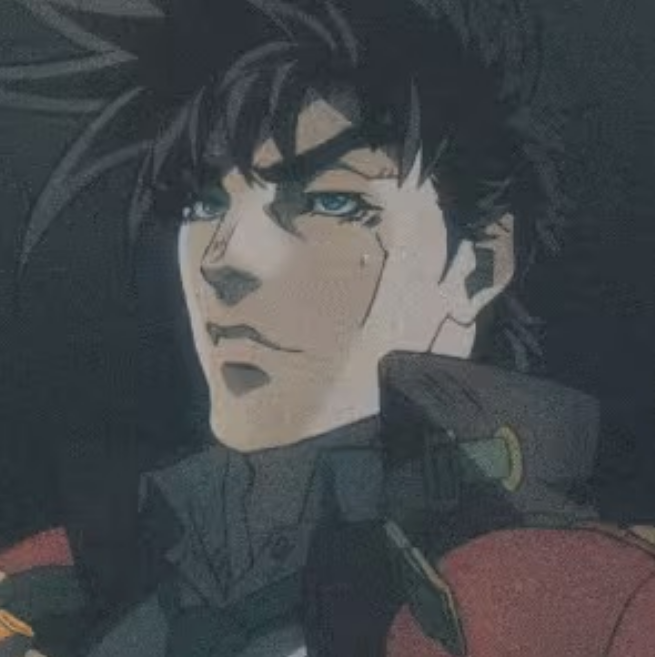
\includegraphics[width=0.06\linewidth]{p2.png}}
\renewcommand{\headrulewidth}{0.4pt}
\renewcommand{\footrulewidth}{0.4pt}

\begin{document}

\begin{center}
\Large\textbf{2014哈工大硕士考试试题：805物理光学}
\end{center}





\section*{一、填空题（20分）}
\begin{enumerate}
    \item 圆偏振光通常分为\_\_\_\_\_和\_\_\_\_\_两种。
    \item \_\_\_\_\_称为波阵面。
    \item 发生全反射的条件是\_\_\_\_\_。，全反射现象的特点\_\_\_\_\_。
    \item 一束光垂直入射在偏振片$p$上，以入射光线为轴，转动$p$，观察通过$p$的光强的变化过程，若入射光是\_\_\_\_\_，则看到光强不变；若入射光是\_\_\_\_\_，则看到明暗交替变化，有时出现全暗；若入射光是\_\_\_\_\_，则看到光强变化，但不出现全暗。
    \item 采用光程概念的好处是\_\_\_\_\_。
    \item 能够将自然光变为偏振光的器件称为\_\_\_\_\_，检验偏振光的器件称为\_\_\_\_\_。
    \item 点光源发出的光波在晶体中传播时，实际波面是\_\_\_\_\_，波法面是\_\_\_\_\_。
    \item 平行平板产生的是\_\_\_\_\_，楔形平板产生的是\_\_\_\_\_干涉。
\end{enumerate}
\section*{二、名词解释（24分）}
\begin{enumerate}
    \item 条纹对比度
    \item 布儒斯特角
    \item 色散
    \item 波片
    \item 巴比涅原理
    \item 半波损失
    \item 双折射
    \item 光栅
\end{enumerate}
\section*{三、选择题（21分）}
\begin{enumerate}
    \item （重复）观察单缝弗朗合费衍射图样时，单缝宽度减小，屏上中央亮纹宽度将\_\_\_\_\_。\\(A)变宽\quad (B)变窄\quad (C)不变\quad (D)难以确定
    \item （重复）瑞利散射与拉曼散射的主要区别是\_\_\_\_\_\\(A)散射光与入射光强度关系\quad(B)散射光与入射光偏振度关系\quad (C)散射光与入射光相干性关系\quad (D)散射光与入射光波长关系
    \item 在双缝干涉实验中，为使屏上的干涉条纹间距变大，可\_\_\_\_\_。\\(A)把两个缝的宽度稍微调窄\quad(B)改用波长较小的单色光源\quad (C)使屏靠近双缝\quad (D)减小双缝间距
    \item 光可能转变成其他形式能量的物理现象是\_\_\_\_\_。\\(A)干涉\quad(B)衍射\quad(C)色散\quad(D)吸收
    \item 沿$z$轴方向传播的平面简谐电磁波，当电场分量$E$极大时，磁场分量$H$\_\_\_\_\_。\\(A)极大\quad(B)极小\quad(C)常数\quad(D)不确定
    \item （重复）一束光是自然光和线偏振光的混合光，让它垂直通过一偏振片，若以此入射光束为轴旋转偏振光，测得透射光强度最大值是最小值5倍，那么入射光束中自然光和线偏振光的光强比值是\_\_\_\_\_.\\(A)1/2\qquad（B）1/5\qquad（C）1/4\qquad（D）2/3
    \item 在各向异性的晶体中，光波$E$和$D$的方向\_\_\_\_\_。\\(A)一定相同\quad(B)互相垂直\quad(C)不一定相同\quad(D)一定不同
\end{enumerate}
\section*{四、简答题（30分）}
\begin{enumerate}
    \item 什么是空间相干性和时间相干性，他们是怎样产生的？
    \item 简述从自然光获得线偏振光的方法。
    \item 什么是等相面和等幅面？举例说明二者一致和不一致的情况。
    \item 决定光波偏振态的因素有哪些？
    \item 简述等倾圆条纹与牛顿环的异同？
    \item 惠更斯——菲涅尔原理
\end{enumerate}
\section*{五、计算与分析（41分）}
\begin{enumerate}
    \item 如图所示，一根圆柱形光纤的折射率为$n_1=1.55$，包层折射率$n_2=1.48$，求最大孔径角$2u$。
         \begin{figure}[!htb]
                \centering
                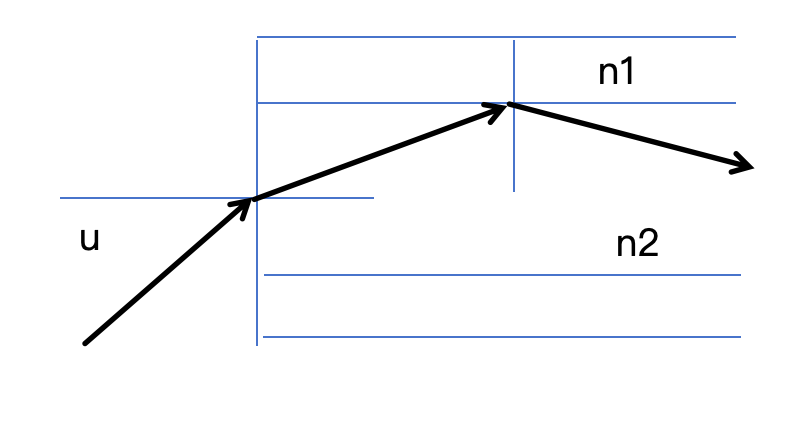
\includegraphics[width=0.7\linewidth]{141.png}
                
          \end{figure}

    \item 已知$F-P$标准距的空气间隔$h=4cm$,两镜面的反射率均为$R=0.891$。另有一反射光栅的刻线面积为$3cm\times3cm$，刻线数为$1200条/mm$。取一级光谱，比较这两个分光元件对波长为$632.8nm$的红光的分光特性。
    \item 一个线偏振光在玻璃中传播时的表达式为：$E_x=0,E_y=0,E_z=(100V/m)(\pi\times10^{14}\times s^{-1}(t-\frac{x}{c})+\frac{\pi}{2})$,求该光的频率，波长，振幅，周期，初相位是多少？
    \item （重复）一束自然光正入射到重叠的两个偏振片上，如果透射光强为入射光强的$3/8$，求两个偏振片的夹角。
    \item （重复） 以纳光观察迈克尔逊干涉条纹，先看到干涉场中12个亮环，且中心是亮点，然后移动一侧反射镜，看到中心消失了10个亮环，此时干涉场中还存在5个亮环。求：
    \begin{enumerate}
        \item 镜面移动的距离
        \item 开始时中心亮斑的级次$k_0$,相对应的等效空气薄膜厚$h_0$
    \end{enumerate}
\end{enumerate}
\section*{六、论述题（10分）}
\begin{enumerate}
    \item 某像质极佳的航天相机光学系统，焦距为$1000mm$，口径直径为$100mm$，工作波段为$0.4-0.6um$,起孔径光阑为圆形，且位于系统的最前端，如果在孔径光阑处放置有两个直径$50mm$开口的挡光片，如图所示，分析光学系统分辨本领的变化情况。
         \begin{figure}[!htb]
                \centering
                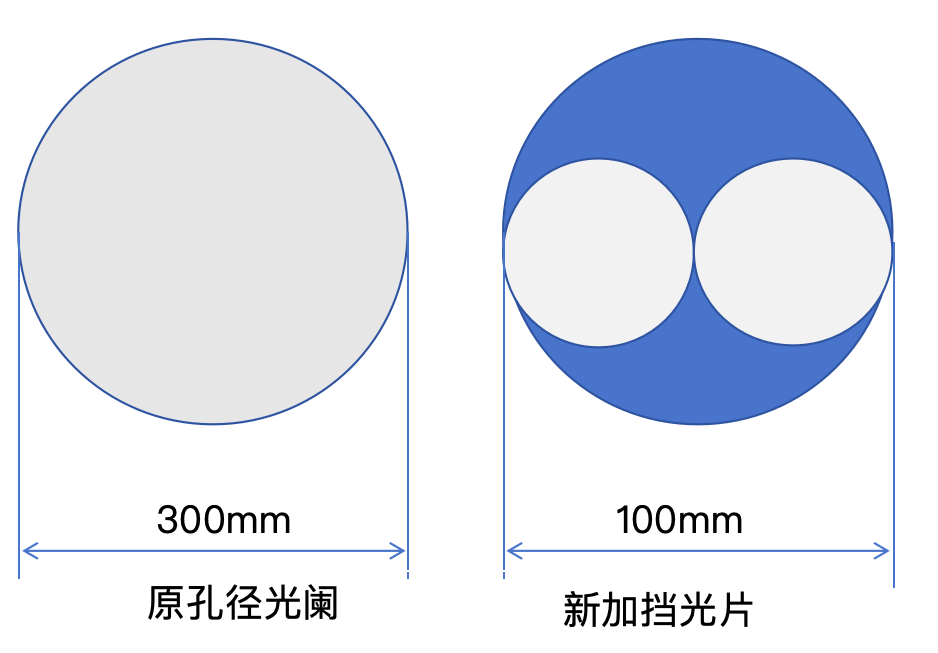
\includegraphics[width=0.7\linewidth]{142.png}
                
          \end{figure}
\end{enumerate}
\end{document}